% Please use the skeleton file you have received in the
% invitation-to-submit email, where your data are already
% filled in. Otherwise please make sure you insert your
% data according to the instructions in PoSauthmanual.pdf
\documentclass[a4paper]{PoS}
\usepackage{subfigure}

\title{Jet Substructure Variables with the SiFCC Detector at 100 TeV}

\ShortTitle{Jet Substructure Variables with the SiFCC Detector at 100 TeV}

\author{\speaker{C.-H Yeh}$^a$,S.V. Chekanov$^b$ ,A.V. Kotwal$^{c}$,J. Proudfoot$^{b}$,S. Sen$^{c}$,N.V. ~Tran$^{d}$,S.-S Yu$^{a}$\\     
     \llap{$^a$}Department of Physics, National Central University\\
     Chung-Li, Taoyuan City 32001, Taiwan\\
     \llap{$^b$}HEP Division, Argonne National Laboratory\\
     9700 S. Cass Avenue, Argonne, IL 60439, USA\\
     \llap{$^c$}Department of Physics, Duke University\\
     Durham, NC 27708, USA\\
     \llap{$^d$}Fermi National Accelerator Laboratory\\
     Batavia, IL 6051, USA\\
     E-mail:  \email{a9510130375@gmail.com},
     \email{chekanov@anl.gov},
     \email{kotwal@phy.duke.edu},
     \email{proudfoot@anl.gov},
     \email{sourav.sen@duke.edu},
     \email{ntran@fnal.gov},
     \email{syu@phy.ncu.edu.tw}}

\abstract{
Future experiments beyond the LHC era
will measure high-momentum bosons ($W$, $Z$, $H$) and top quarks with strongly
collimated decay products that form hadronic jets.
This paper describes the studies  
of the performance of jet substructure variables using 
the Geant4 simulation of a detector designed for  high energy $pp$ collisions at a 100 TeV collider.  
The two-prong jets from Z'$\rightarrow$$WW$ and three-prong jets from Z'$\rightarrow$$t\bar{t}$ are compared with 
the background from light quark jets, assuming  $Z'$ masses in the range 5 -- 40 TeV.   
Our results indicate that the performance of jet-substructure 
reconstruction improves with reducing transverse cell sizes of a hadronic calorimeter 
from $\Delta \eta \times \Delta \phi = 0.1\times0.1$
to $0.022\times0.022$.} 

\FullConference{The 39th International Conference on High Energy Physics (ICHEP2018)\\
		4-11 July, 2018\\
		Seoul, Korea}


\begin{document}

Future high-energy experiments, such as FCC-hh and SppC, 
will measure high-momentum bosons ($W$, $Z$, $H$) and top quarks 
with strongly collimated decay products that form hadronic jets. This leads to many
challenges for detector technologies.  In particular, reconstruction of jet substructure  variables for boosted jets with transverse
momentum above 10~TeV
requires appropriate  cell sizes of hadronic
calorimeters  (HCALs). In order to estimate 
transverse segmentation  
of HCALs for very boosted objects at future experiments, 
we used a FCC-like detector geometry,
a software based on Geant4 simulation and Monte Carlo event samples as described in~\cite{Chekanov:2016ppq}.
 
In this study we simulated the $Z'$ bosons with the center-of-mass energies (c.m.) at 5, 10, 20, and 40 TeV. These particles are forced to decay to two light-flavor jets ($q\bar{q}$) as background, $W W$ or $t\bar{t}$ as signal, where $W$($\rightarrow q\bar{q}$) and $t$($ \rightarrow  W^+\>b \rightarrow q\bar{q} b$) decay hadronically. We use different configurations of HCAL geometry to see whether the smallest configuration can give the best separation power to distinguish signal from background in different jet substructures. We draw the receiver operating characteristic (ROC) curves to quantify the detector performance and find out the cell size that can give the best separation power.

We used several jet substructure variables, including $N$-subjettiness~\cite{Thaler:2010tr} and energy correlation function~\cite{Larkoski:2013eya} to study. The signals considered are $Z'\rightarrow WW$ ($\tau_{21}$,$C_2^1$) and $Z' \rightarrow t\bar{t}$ ($\tau_{32}$). Figure~\ref{1} shows the ROC curves for the $\tau_{21}$~\cite{Thaler:2010tr} using three HCAL sizes for jets at 20 TeV. For all of them, the smallest detector cell size ($1\times1~\mathrm{cm}^2$, or $\Delta \eta \times \Delta \phi = 0.005\times0.005$) does not have the best separation power. It is interesting to note that at very large c.m. energies, the large detector cell sizes have a better separation power than the smallest cell size in most of cases. 

In conclusion, the  performance 
of a  HCAL with 
$\Delta \eta \times \Delta \phi = 0.022\times0.022$ (or $5\times5$ cm$^2$)cells is, in most cases,
better than for $0.1\times0.1$ (or $20\times20$ cm$^2$) cells.
Therefore, this study confirms the  baseline SiFCC detector geometry \cite{Chekanov:2016ppq}
that uses $\Delta \eta \times \Delta \phi = 0.022\times0.022$ HCAL cells.

\begin{figure}
\begin{center}
 %\subfigure[Soft drop mass with $\beta=0$ and 20 TeV] {
% 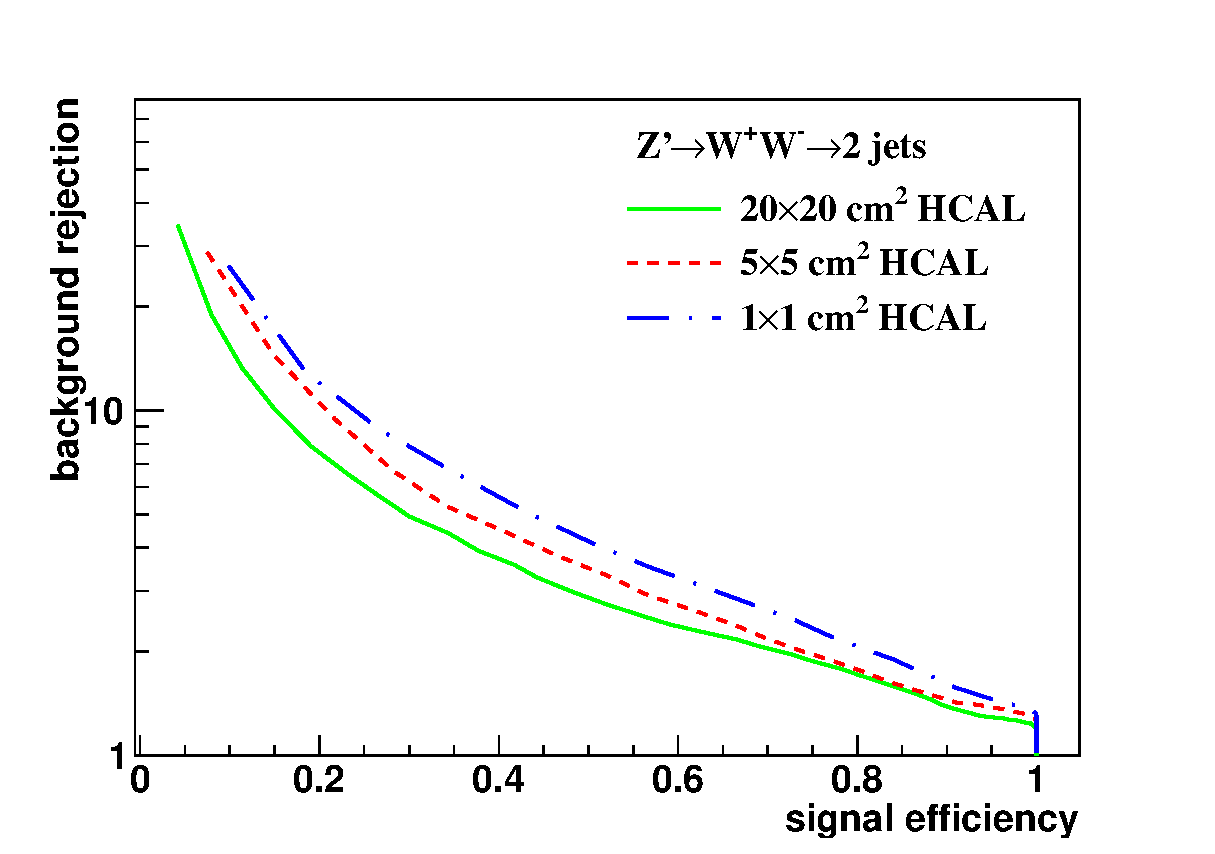
\includegraphics[width=0.35\textwidth]{A_Cluster_mass_mmdt_20tev_eff_1_central_fix_at_Median_bin_ww_qq_log_no_UOF.eps}
 %}
 \includegraphics[width=0.35\textwidth]{Rawhit_05GeV_tau21_20tev_eff_1_New2_after_cut_25bins_no_UOF_new_75pa.eps}
\end{center}
\caption{$\tau_{21}$ with 20 TeV.}
\label{1}
\end{figure}
\begin{thebibliography}{99}
\bibitem{Chekanov:2016ppq} 
  S.~V.~Chekanov, M.~Beydler, A.~V.~Kotwal, L.~Gray, S.~Sen, N.~V.~Tran, S.-S.~Yu and J.~Zuzelski,
  \emph{Initial performance studies of a general-purpose detector for multi-TeV physics at a 100 TeV pp collider},
  \emph{JINST} {\bf 12}, no. 06, P06009 (2017)
  doi:10.1088/1748-0221/12/06/P06009
  [arXiv:1612.07291 [hep-ex]].
%%%
\bibitem{Thaler:2010tr} 
  J.~Thaler and K.~Van Tilburg,
  \emph{JHEP} {\bf 1103}, 015 (2011)
  JHEP 03 (2011) 015, 
  [arXiv:1011.2268].
%%%
\bibitem{Larkoski:2013eya} 
  A.~J.~Larkoski, G.~P.~Salam and J.~Thaler,
  \emph{JHEP} {\bf 1306}, 108 (2013)
  JHEP 06 (2013) 108
  [arXiv:1305.0007].

%%%
\end{thebibliography}

\end{document}
